\newpage
\section{GeoPoly Framework}
\label{sec:algo}
{\sc GeoPoly} is an approach which exploits analyst's implicit feedback (i.e., mouse moves) to highlight few interesting points as future analysis directions. Algorithm \ref{algo:main} summarizes the principled steps of our approach.

\begin{algorithm}[t]
\DontPrintSemicolon
\KwIn{Current time $t_c$, mouse move points $\mathcal{M}$}
\KwOut{Highlights $\mathcal{P}_k$}
$\mathcal{S} \gets \mathit{find\_interesting\_dense\_regions}(t_c,\mathcal{M})$\label{ln:dense}\;
$\mathcal{P}_s \gets \mathit{match\_points}(\mathcal{S}, \mathcal{P})$\label{ln:match}\;
$F \gets \mathit{update\_feedback\_vector}(F, \mathcal{P}_s)$\label{ln:update}\;
$\mathcal{P}_k \gets \mathit{get\_highlights}(\mathcal{P}, F)$\label{ln:highlight}\;
\Return{$\mathcal{P}_k$}\; 
\caption{{\sc GeoPoly} Algorithm}
\label{algo:main}
\end{algorithm}

\vspace{2pt}
The algorithm begins by mining the set of mouse move points $\mathcal{M}$ in the interaction layer to discover one or several Interesting Dense Regions, abbr., IDRs, in which most analyst's interactions occur (line \ref{ln:dense}). Then it matches the spatial points $\mathcal{P}$ with IDRs using Equation \ref{eq:reverse} in order to find points inside each ragion (line \ref{ln:match}). The attributes of resulting points will be exploited to update the analyst's feedback vector~$F$~(line \ref{ln:update}). The updated vector $F$ will then be used to find $k$ highlights (line \ref{ln:highlight}). These steps ensure that the final highlights reflect analyst's implicit interests. We detail each step as follows.

\subsection{Interesting Dense Regions}
The objective of this step is to obtain one or several regions in which the analyst has expressed her implicit feedback. There are two observations for such regions.

\vspace{2pt}
\noindent $\blacksquare$ {\bf Observation 1.} We believe that a region appeals more interesting to the analyst if it is denser, i.e., the analyst moves her mouse in that region several times.

\vspace{2pt}
\noindent $\blacksquare$ {\bf Observation 2.} It is possible that the analyst moves her mouse everywhere in the map. This should not signify that everywhere in the map has the same significance.

\vspace{2pt}
Following our observations, we propose Algorithm \ref{algo:dense} for mining IDRs. We add points to $\mathcal{M}$ only every $200ms$ to prevent adding redundant points.  Following Observation 1 and in order to mine the recurring behavior of the analyst, the algorithm begins by partitioning the set $\mathcal{M}$ into $g$ fixed-length consecutive segments $\mathcal{M}_0$ to $\mathcal{M}_g$. The first segment starts at time zero (where the system started), and the last segment ends at $t_c$, i.e., the current time. Following Observation 2, we then find dense clusters in each segment of $\mathcal{M}$ using a variant of DB-SCAN~\cite{Ester:1996} approach. Finally, we return intersections among those clusters as IDRs.

\vspace{2pt}
For clustering points in each time segment (i.e., line \ref{ln:mine} of Algorithm~\ref{algo:dense}), we use ST-DBSCAN~\cite{Birant:2007}, a space-aware variant of DB-SCAN for clustering points based on density. For each subset of mouse move points $\mathcal{M}_i$, $i \in [0,g]$, ST-DBSCAN begins with a random point $m_0 \in \mathcal{M}_i$ and collects all density-reachable points from $m_0$ using a distance metric. As mouse move points are the 2-dimensional pixel space (i.e., the display), we choose euclidean distance as the distance metric. If $m_0$ turns out to be a core object, a cluster will be generated. Otherwise, if $m_0$ is a border object, no point is density-reachable from $m_0$ and the algorithm picks another random point in $\mathcal{M}_i$. The process is repeated until all of the points have been processed.

\vspace{2pt}
Once clusters are obtained for all subsets of $\mathcal{M}$, we find their intersections to locate recurring regions (line \ref{ln:poly}). To obtain intersections, we need to clearly define the spatial boundaries of each cluster. Hence for each cluster, we discover its corresponding polygon that covers the points inside. For this aim, we employ Quickhull algorithm, a quicksort-style method which computes the convex hull for a given set of points in a 2D plane~\cite{Barber:1996}.
% We analysed other different approaches~\cite{Bevis1989,DUCKHAM2008,FADILI2004,ARAMPATZIS2006,Galton2006} to generate regions from clustered points, however we decided to use the Quickhull  algorithm~\cite{Barber:1996}, that presented more appropriated to our proposed solution.

\begin{figure*}[t]
\centering
   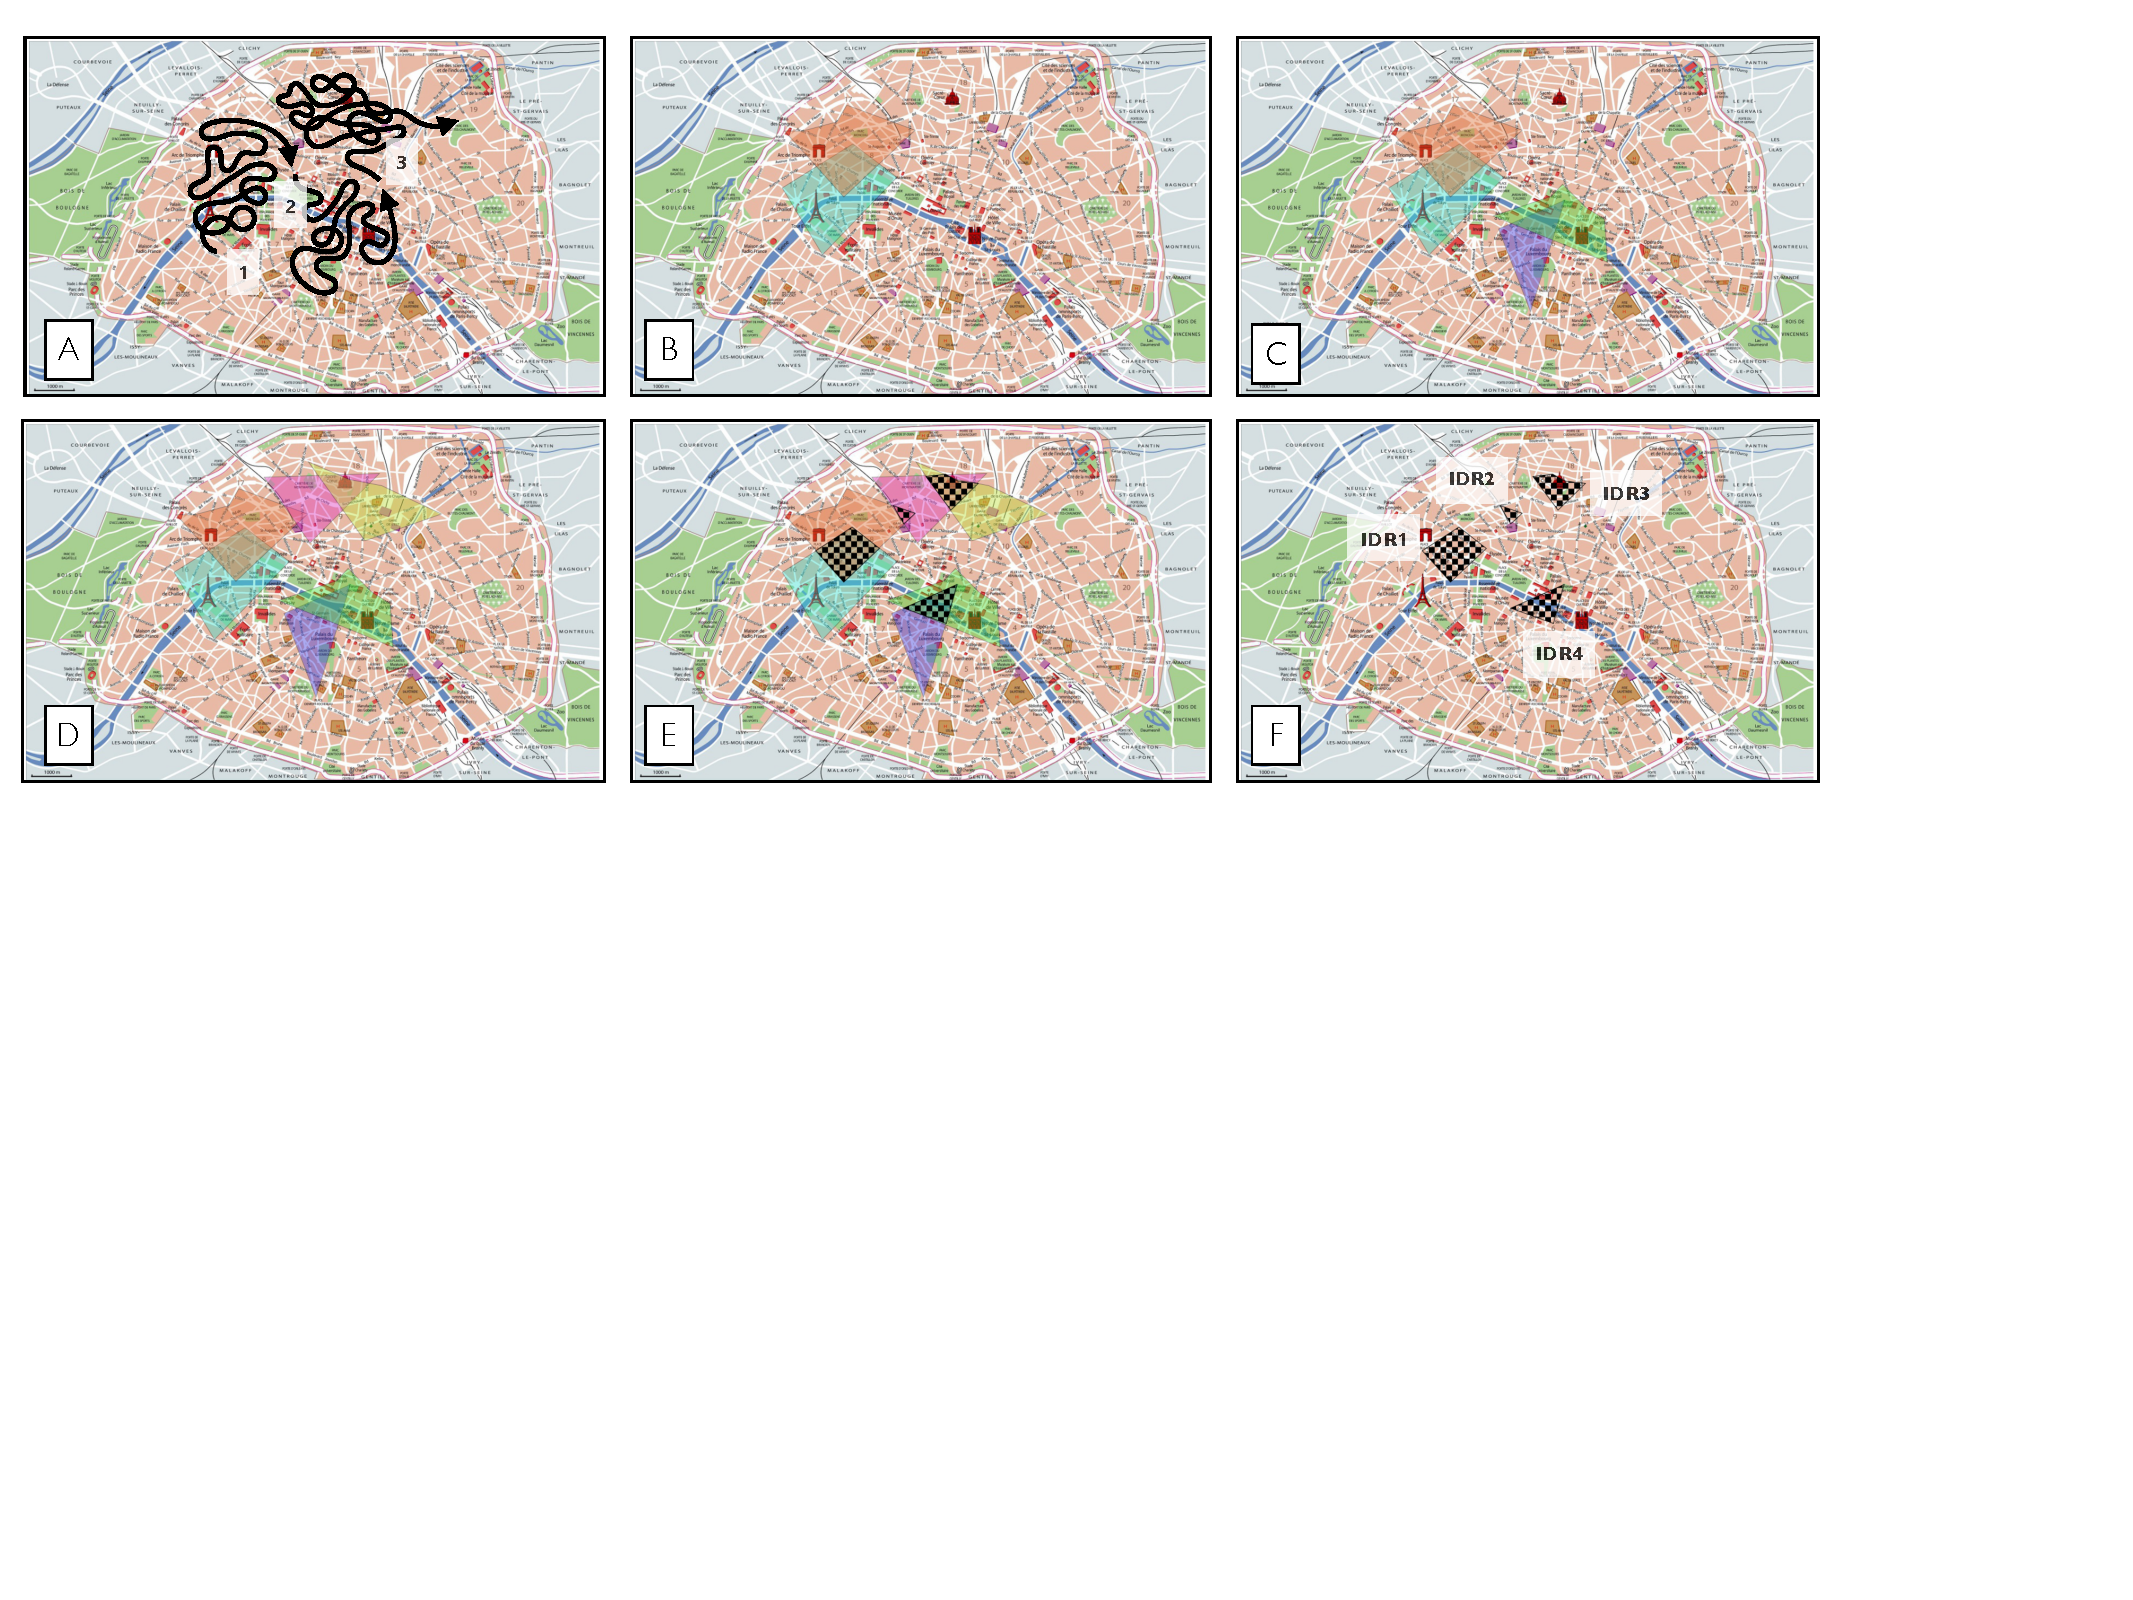
\includegraphics[width=\textwidth]{imgs/regions}
  \caption{The process of finding IDRs on Airbnb dataset.}
  \label{fig:regions}
\end{figure*}

\begin{algorithm}[t]
\DontPrintSemicolon
\KwIn{Current time $t_c$, mouse move points $\mathcal{M}$}
\KwOut{IDRs $\mathcal{S}$}
$\mathcal{S} \gets \emptyset$\;
$g \gets ${\em number of time segments}\;
\For{$i \in [0,g]$}
{
       $\mathcal{M}_i \gets \{m = \langle x,y,t \rangle | (\frac{t_c}{g} \times i) \leq t \leq (\frac{t_c}{g} \times (i+1))\}$\;
       $\mathcal{C}_i \gets \mathit{mine\_clusters}(\mathcal{M}_i)$\label{ln:mine}\;
       $\mathcal{O}_i \gets \mathit{find\_ploygons}(\mathcal{C}_i)$\label{ln:poly}\;
}
\lFor{$\mathcal{O}_i, \mathcal{O}_j$ where $i,j \in [0,g]$ and $i \neq j$}
{
       $\mathcal{S}.\mathit{append}(\mathit{intersect}(\mathcal{O}_i, \mathcal{O}_j))$
}
\Return{$\mathcal{S}$}\; 
\caption{Find Interesting Dense Regions (IDRs)}
\label{algo:dense}
\end{algorithm}

\begin{figure}[t]
\centering
   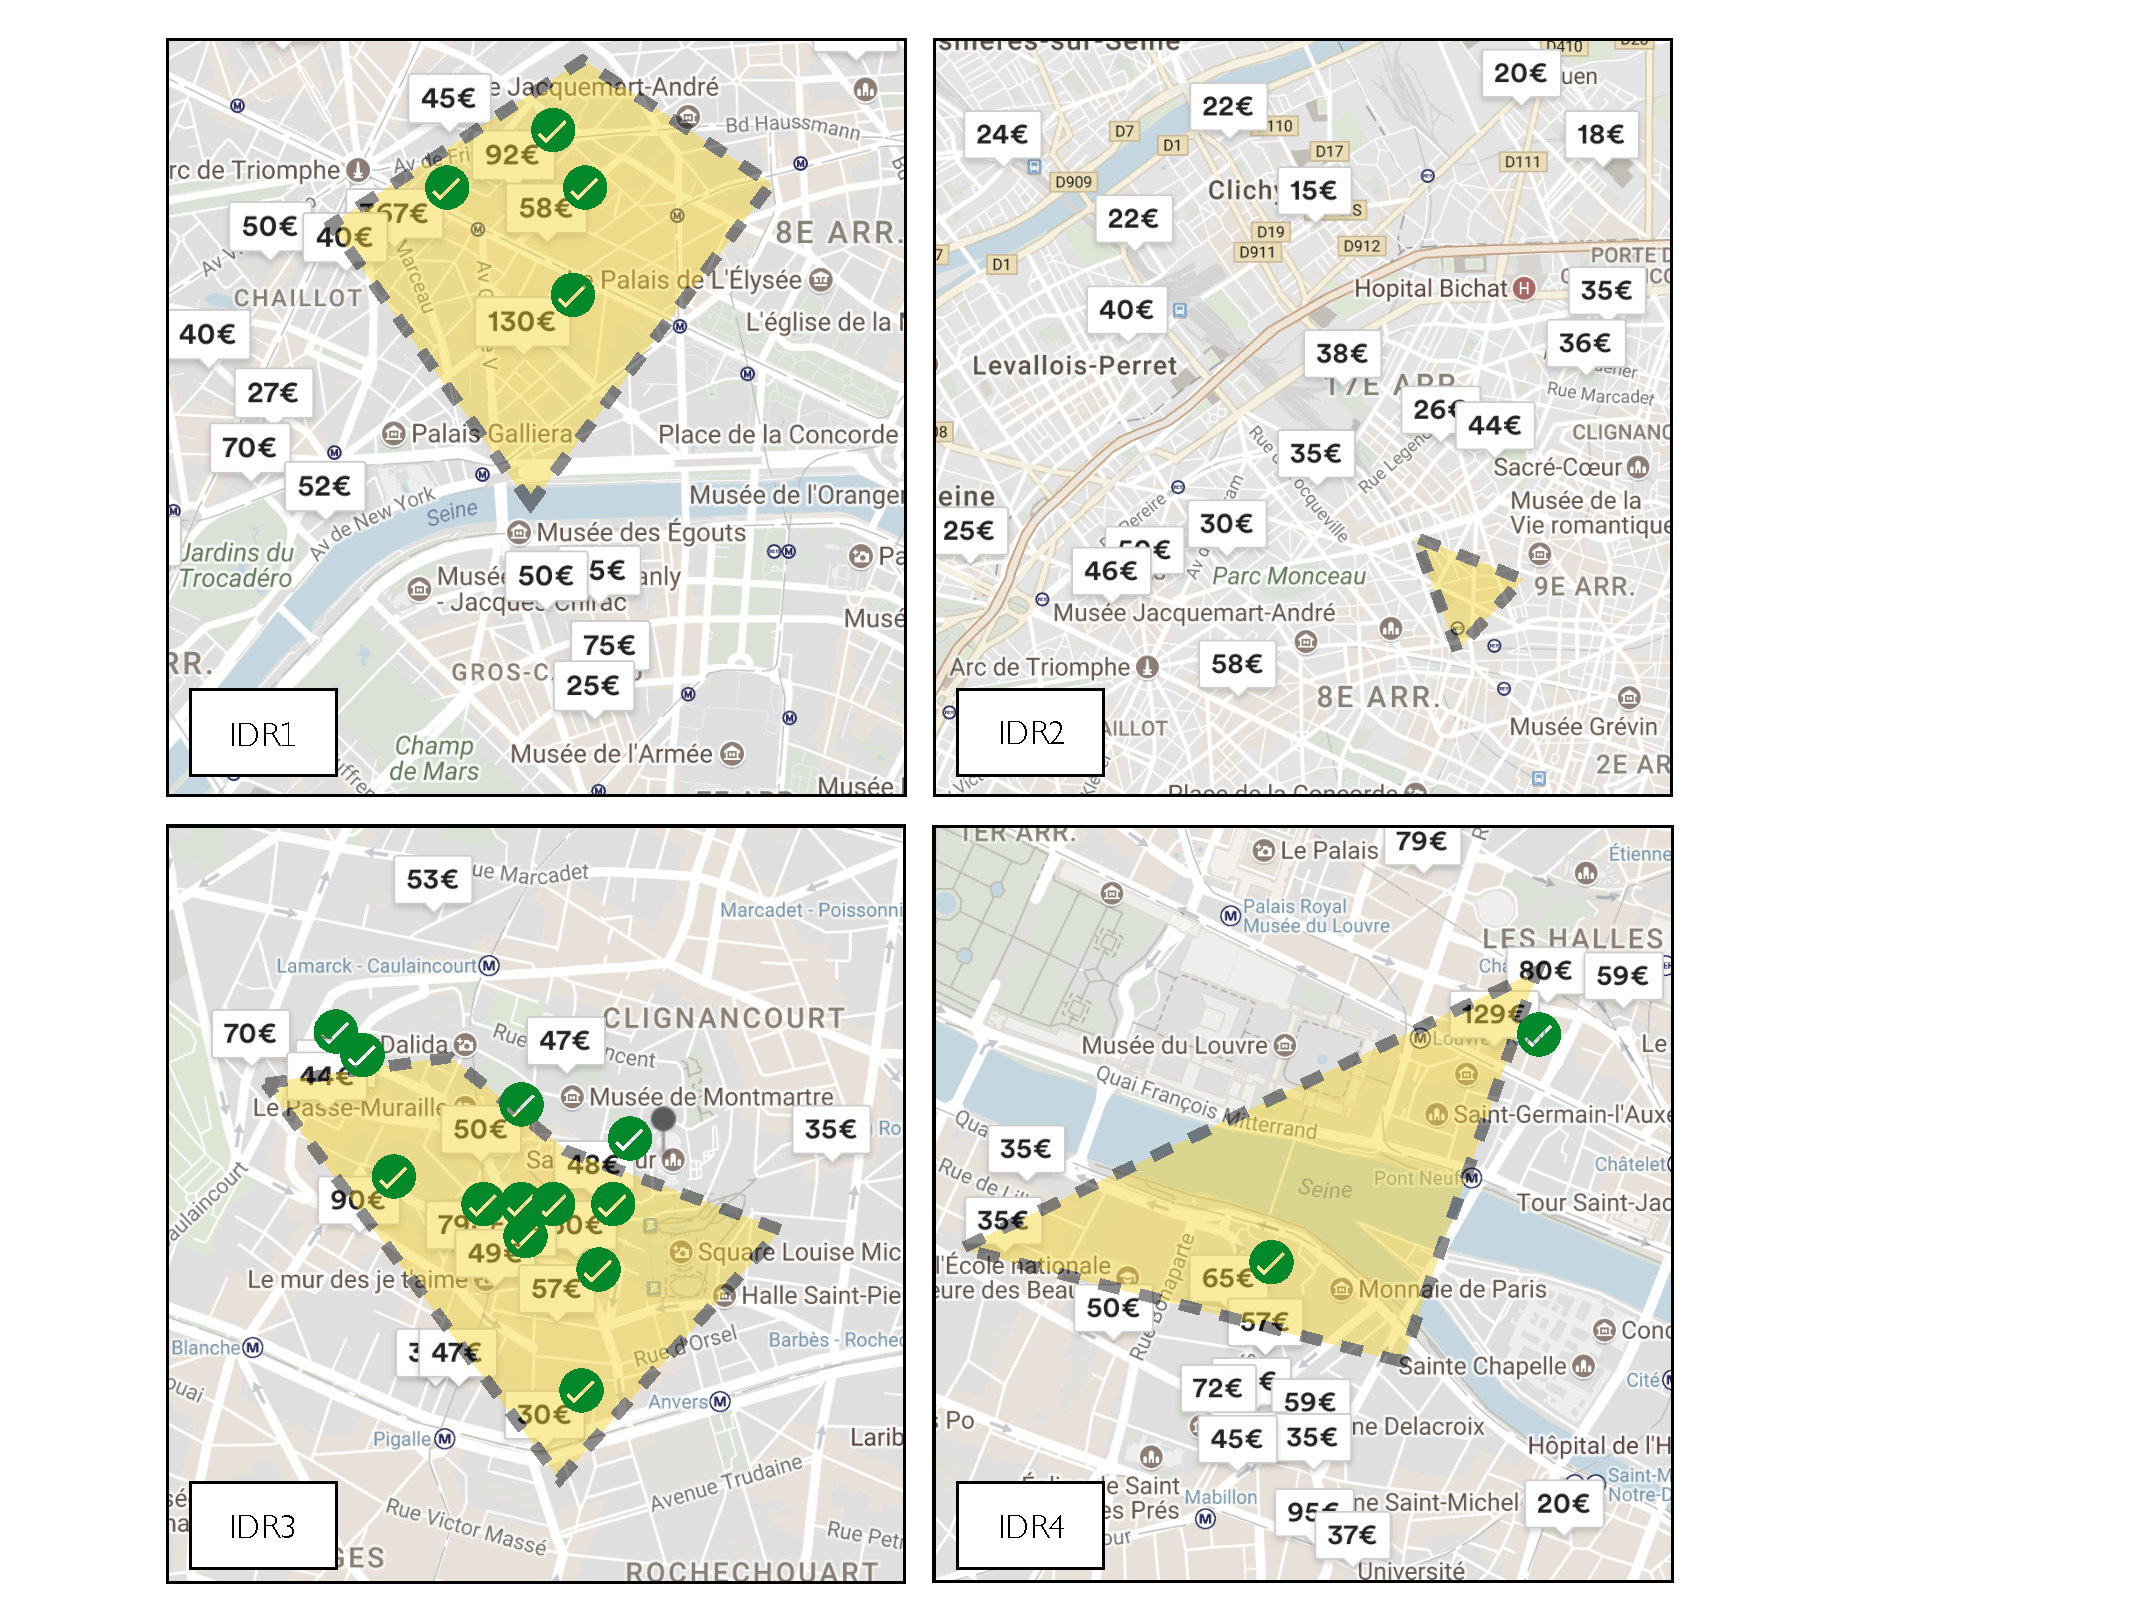
\includegraphics[width=\columnwidth]{imgs/match}
  \caption{Matching points for IDR1 to IDR4.}
  \label{fig:match}
\end{figure}

\vspace{2pt}
We describe the process of finding IDRs in an example. Figure \ref{fig:regions} shows the steps that Ben\'icio follows in our running example to explore home-stays in Paris. Figure \ref{fig:regions}.A shows mouse movements of Ben\'icio in different time stages. In this example, we consider $g = 3$ and capture Ben\'icio's feedback in three different time segments (progressing from Figures \ref{fig:regions}.B to \ref{fig:regions}.D). It shows that Ben\'icio started his search around Eiffel Tower and Arc de Triomphe (Figure \ref{fig:regions}.B) and gradually showed interest in south (Figure \ref{fig:regions}.C) and north (Figure \ref{fig:regions}.D) as well. All intersections between those clusters are discovered (hatching regions in Figure \ref{fig:regions}.E) which will constitute the set of IDRs (Figure \ref{fig:regions}.F), i.e., IDR1 to IDR4.

\subsection{Matching Points}
Being a function of mouse move points, IDRs are discovered in the interaction layer. We then need to find out which points in $\mathcal{P}$ fall into IDRs, hence forming the subset $\mathcal{P}_s$. We employ Equation \ref{eq:reverse} to transform those points from the spatial layer to the interaction layer. Then a simple ``spatial containment'' function can verify which points fit into the IDRs. Given a point $p$ and an IDR $r$, a function $\mathit{contains}(p,r)$ returns ``true'' if $p$ is inside $r$, otherwise ``false''. In our case, we simply use the implementation of $\mathit{ST\_Within}(p,r)$ module in PostGIS\footnote{\it https://postgis.net/docs/manual-dev/ST\_Within.html}, i.e., our underlying spatial DBMS which hosts the data.

\vspace{2pt}
In the vanilla version of our spatial containment function, all points should be checked against all IDRs. Obviously, this depletes the execution time. To prevent the exhaustive scan, we employ Quadtrees in a two-step approach.

\vspace{4pt}
\noindent $\blacksquare$ In an offline process, we build a Quadtree index for all points in $\mathcal{P}$. We record the membership relations of points and cells in the index.

\vspace{2pt}
\noindent $\blacksquare$ When IDRs are discovered, we record which cells in the Quadtree index intersect with IDRs. As we often end up with few IDRs, the intersection verification performs fast. Then for matching points, we only check a subset which is inside the cells associated to IDRs and ignore the points outside. This leads to a drastic pruning of points in $\mathcal{P}$.

\vspace{4pt}
We follow our running example and illustrate the matching process in Figure \ref{fig:match}. In the Airbnb dataset, points are home-stays which are shown with their nightly price on the map. We observe that there exist many matching points with IDR3 and absolutely no matching point for IDR2. For IDR4, although there exist many home-stays below the region, we never check their containment, as they belong to a Quadtree cell which doesn't intersect with the IDR. 

\subsection{Updating Analyst Feedback Vector}
The set of matching points $\mathcal{P}_s$ (line \ref{ln:match} of Algorithm \ref{algo:main}) depicts the implicit preference of the analyst. We keep track of this preference in a feedback vector $F$. The vector is initialized by zero, i.e., the analyst has no preference at the beginning. We update $F$ using the attributes of the points in $\mathcal{P}_s$.

\vspace{2pt}
We consider an {\em increment value} $\delta$ to update $F$. If $p \in \mathcal{P}_s$ gets $v_1$ for attribute $a_1$, we augment the value in the $F$'s cell of $\langle a_1, v_1 \rangle$ by $\delta$. Note that we only consider incremental feedback, i.e., we never decrease a value in $F$.

\vspace{2pt}
We explain the process of updating the feedback vector using a toy example. Given the four matched points in IDR1 (Figure \ref{fig:match}) with prices 130\euro, 58\euro, 92\euro\ and 67\euro, we want to update the vector $F$ given those points. Few attributes of these points are mentioned in Table \ref{tbl:attribs}. In practice, there are often more than 50 attributes for points. The cells of $F$ is illustrated in the first column of Table \ref{tbl:feedback}. As three points get the value ``1'' for the attribute ``\#Beds'', then the value in cell $\langle$\#Beds,1$\rangle$ is augmented three times by $\delta$. The same process is repeated for all attribute-values of points in $\mathcal{P}_s$. Note that all cells of $F$ are not necessarily touched in the feedback update process. For instance, in the above example, 5 cells out of 12 remain unchanged.

\vspace{2pt}
By specifying an increment value, we can materialize the updates and normalize the vector using a Softmax function. We always normalize $F$ in a way that all cell values sum up to $1.0$. Given $\delta = 1.0$, the normalized values of the $F$ vector is illustrated in the third column of Table \ref{tbl:feedback}. Higher values of $\delta$ increase the influence of feedbacks.

\vspace{2pt}
The normalized content of the vector $F$ captures the implicit preferences of the analyst. For instance, the content of $F$ after applying points in IDR1 shows that the analyst has a high interest in having a balcony in her home-stay, as her score for the cell $\langle$Balcony,Yes$\rangle$ is 0.25, i.e., the highest among other cells. This reflects the reality as all points in IDR1 has balcony. Note that although we only consider positive feedback, the Softmax function lowers the values of untouched cells once other cells get rewarded.

\vspace{2pt}
An important consideration in interpreting the vector $F$ is that the value ``0'' does not mean the lowest preference, but {\em irrelevance}. For instance, consider the cell $\langle$Rating,2$\rangle$ in Table \ref{tbl:feedback}. The value ``0'' for this cell shows that the analyst has never expressed her implicit feedback on this facet. It is possible that in future iterations, the analyst shows interest in a 2-star home-stay (potentially thanks to its price), hence this cell gets a value greater than zero. However, cells with lower preferences are identifiable with non-zero values tending to zero. For instance, the value 0.06 for the cell $\langle$Rating,4$\rangle$ shows a lower preference towards 4-star home-stays comparing to the ones with 5 stars, as only one point in $\mathcal{P}_s$ is rated 4 in IDR1.

\begin{table}[t]
\centering
\caption{Attributes of points in IDR1.}
\label{tbl:attribs}
\begin{tabular}{|c|c|c|c|c|c|}
\hline
\textbf{ID} & \textbf{Price} & \textbf{\#Beds} & \textbf{Balcony} & \textbf{Air-cond.} & \textbf{Rating} \\ \hline
1                     & 130\euro           & 1               & Yes           & Yes                & 5/5             \\ \hline
2                     & 58\euro            & 1               & Yes           & No                 & 5/5             \\ \hline
3                     & 92\euro            & 2               & Yes           & No                 & 5/5             \\ \hline
4                     & 67\euro            & 1               & Yes           & No                 & 4/5             \\ \hline
\end{tabular}
\end{table}

\begin{table}[t]
\centering
\caption{Updating Analyst Feedback Vector}
\label{tbl:feedback}
\begin{tabular}{|c|c|c|}
\hline
\textbf{Attribute-value}               & \textbf{Applying IDR 1} & \textbf{Normalized} \\ \hline
$\langle$\#Beds,1$\rangle$                   & $+3\delta$                       & 0.19                 \\ \hline
$\langle$\#Beds,2$\rangle$                 & $+\delta$                       & 0.06                 \\ \hline
$\langle$\#Beds,+2$\rangle$                  & {\em (no update)}                       & 0.00                    \\ \hline
$\langle$Balcony,Yes$\rangle$                   & $+4\delta$                      & {\bf 0.25}                 \\ \hline
$\langle$Balcony,No$\rangle$                    & {\em (no update)}                        & 0.00                    \\ \hline
$\langle$Air-cond.,Yes$\rangle$               & $+\delta$                       & 0.06                 \\ \hline
$\langle$Air-cond.,No$\rangle$                & $+3\delta$                       & 0.19                 \\ \hline
$\langle$Rating,1$\rangle$                    & {\em (no update)}                       & 0.00                    \\ \hline
$\langle$Rating,2$\rangle$                     & {\em (no update)}                        & 0.00                    \\ \hline
$\langle$Rating,3$\rangle$                    & {\em (no update)}                        & 0.00                   \\ \hline
$\langle$Rating,4$\rangle$                   & $+\delta$                       & {\bf 0.06}                 \\ \hline
$\langle$Rating,5$\rangle$                     & $+3\delta$                      & 0.19                 \\ \hline
\end{tabular}
\end{table}

\subsection{Generating Highlights}
The ultimate goal of \sgg\ is to highlight $k$ points to guide analysts in analyzing their spatial data. The updated feedback vector $F$ is the input to the highlighting phase. We assume that points in IDRs are already investigated by the analyst. Hence our search space for highlighting is $\mathcal{P} - \mathcal{P}_s$.

\vspace{2pt}
We seek two properties in $k$ highlights, i.e., {\em similarity} and {\em diversity}. First, highlights should be in the same direction of the analyst's implicit feedback, hence similar to the vector~$F$. The similarity between a point $p \in \mathcal{P}$ and the vector~$F$ is defined as follows.

\begin{equation}
       \label{eq:rel}
       \mathit{similarity}(p,F) = \mathit{avg}_{a \in \mathcal{A}}(\mathit{sim(p, F, a)})
\end{equation}

The $\mathit{sim}()$ function can be any function such as Jaccard and Cosine. Each attribute can have its own similarity function (as string and integer attributes are compared differently.) Then $\mathit{sim}()$ works as an overriding-function which provides encapsulated similarity computations for any type of attribute.

\vspace{2pt}
Second, highlighted points should also represent distinct directions so that the analyst can observe different aspects of data and decide based on the big picture. Given a set of points $\mathcal{P}_k = \{ p_1, p_2 \dots p_k \} \subseteq {\cal P}$, we define {\em diversity} as follows.

\begin{equation}
       \label{eq:divs}
       \mathit{diversity}(\mathcal{P}_k) = \mathit{avg}_{\{p, p'\} \subset \mathcal{P}_k | p \neq p' } \mathit{distance}(p,p')
\end{equation} 

The function $\mathit{distance}(p,p')$ operates on geographical coordinates of $p$ and $p'$ and can be considered as any distance function of Minkowski distance family. However, as distance computations are done in the spherical space, a natural choice is to employ Haversine distance shown in Equation~\ref{eq:harvestine}.

\begin{dmath}
       \label{eq:harvestine}
       distance(p,p') = acos(cos(p.\mathit{lat}) \times cos(p'.\mathit{lat}) \times cos(p.\mathit{lon})) \times cos(p'.\mathit{lon}) + cos(p.\mathit{lat}) \times sin(p'.\mathit{lat}) \times cos(p.\mathit{lon}) \times sin(p'.\mathit{lon}) + sin(p.\mathit{lat}) \times sin(p'.\mathit{lat})) \times earth\_radius
\end{dmath}

Algorithm \ref{algo:geoh} describes our approach for highlighting $k$ similar and diverse points.
We propose a best-effort greedy approach to efficiently compute highlighted points. We consider an offline step followed by the online execution of our algorithm.

\vspace{2pt}
In order to speed up the similarity computation in the online execution, we pre-compute an inverted index for each single point $p \in {\cal P}$ in the offline step (as is commonly done in the Web search). Each index ${\cal L}_p$ for the point $p$ keeps all other points in ${\cal P}$ in decreasing order of their similarity with $p$.

\vspace{2pt}
The first step of Algorithm \ref{algo:geoh} is to find the most similar point to $F$, so-called $p^*$. The point $p^*$ is the closest possible approximation of $F$ in order to exploit pre-computed similarities. The algorithm makes sequential accesses to ${\cal L}_{p^*}$ (i.e., the inverted index of the point $p^*$) to greedily maximize diversity. Algorithm \ref{algo:geoh} does not sacrifice efficiency in price of value. We consider a {\em time limit} parameter which determines when the algorithm should stop seeking maximized diversity. Scanning inverted indexes guarantees the similarity maximization even if time limit is chosen to be very restrictive. Our observations with several spatial datasets show that we achieve the diversity of more than $0.9$ with time limit set to $200ms$.

% %\noindent{\bf Context.} 

\begin{algorithm}[t]
\DontPrintSemicolon
\KwIn{Points $\mathcal{P}$, Feedback vector $F$, $k$, $\mathit{time\_limit}$}
\KwOut{$\mathcal{P}_k$}
$p^* \gets \mathit{max\_sim\_to}(\mathcal{P},F)$\;
$\mathcal{P}_k \gets \mathit{top\_k}(\mathit{{\cal L}_{p^*}},k)$\label{ln:topk}\;
$p_{next} \gets get\_next(\mathit{{\cal L}_{p^*}})$\;\label{cd:getnext}
\While{$\mathit{time\_limit}$ $not$ $exceeded$}
       {\label{cd:beginwhile}
       \For{$p_{current} \in {\cal P}_k$}
              {
              \If{$\mathit{diversity\_improved}({\cal P}_k,p_{next},p_{current})$}
                     {\label{cd:betterdiv}
                     ${\cal P}_k \gets \mathit{replace}({\cal P}_k,p_{next},p_{current})$\;
                            $break$\;
                     }
              }
              $p_{next} \gets get\_next(\mathit{{\cal L}_{p^*}})$\;}\label{cd:endwhile}
       \Return{${\cal P}_k$}\; 
       \caption{Get $k$ similar and diverse highlights $\mathit{get\_highlights}()$}
       \label{algo:geoh}
\end{algorithm}

\vspace{2pt}
In line \ref{ln:topk} of Algorithm \ref{algo:geoh}, $\mathcal{P}_k$ is initialized with the $k$ highest ranking points in ${\cal L}_{p^*}$. Function $get\_next({\cal L}_{p^*})$ (line \ref{cd:getnext}) returns the next point $p_{next}$ in ${\cal L}_{p^*}$ in sequential order. Lines \ref{cd:beginwhile} to \ref{cd:endwhile} iterate over the inverted indexes to determine if other points should be considered to increase diversity while staying within the time limit.

\vspace{2pt}
The algorithm looks for a candidate point $p_{\mathit current} \in {\cal P}_k$ to replace in order to increase diversity. The boolean function $\mathit{diversity\_improved}()$ (line \ref{cd:betterdiv}) checks if by replacing $p_{current}$ by $p_{next}$ in ${\cal P}_k$, the overall diversity of the new ${\cal P}_k$ increases.



% Algorithm \ref{algo:geoh} modifies the original {\sc Highlighter} proposal presented in GeoGuide \cite{Omidvar:2017} approach .  
% The original begins by retrieving the most relevant points to $p$ by simply retrieving the $k$ highest ranking points in ${\cal L}_p$ (line \ref{cd:gettopk}) and function $get\_next({\cal L}_p)$ (Line \ref{cd:getnext}) returns the next point $p_{next}$ in ${\cal L}_p$ in sequential order. Line \ref{cd:empty_regions} initialize the set of points that will be retrieved by the highlighted regions. At the beginning we consider that there is no preferred regions. So, the sets ${\cal S}_{rp}$ and ${\cal S}_{p}$  are the same. Lines \ref{cd:beginwhile} to \ref{cd:endwhile} iterate over the inverted indexes to determine if other points should be considered to increase diversity while staying within the time limit and not violating the relevance threshold with the selected point. %Since points in ${\cal L}_g$ are sorted on decreasing relevance with $p$, the algorithm can safely stop as soon as the relevance condition is violated (or if the time limit is exceeded).

% The algorithm then looks for a candidate point $p_{current} \in {\cal S}_p$ to replace in order to increase diversity. If the candidate point is presented in a region $r$ (line \ref{cd:point_in_region}), the point is included in ${\cal S}_{rp}$, considering the boolean function $\mathit{diversity\_improved}()$ (line \ref{cd:betterdiv}). This function checks if by replacing $p_{current}$ by $p_{next}$ in ${\cal S}_p$, the overall diversity of the new ${\cal S}_p$ increases. If the point is not in the preferred region, it is included into ${\cal S}_p$.